% Generated 2021-02-25 13:56:52 +0530
\subsection{CoordinateSystems} \label{sec:CoordinateSystems}


This section provides semantic information for the \block{CoordinateSystem} model.

\begin{figure}[ht]
  \centering
    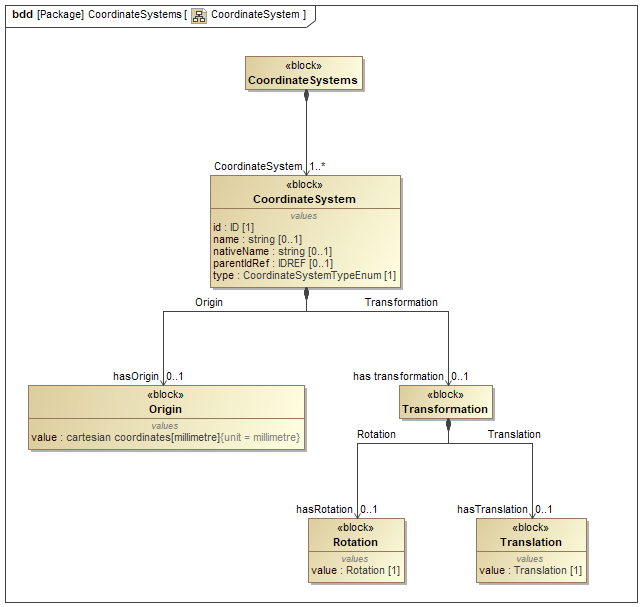
\includegraphics[width=1.0\textwidth]{figures/CoordinateSystem.png}
  \caption{CoordinateSystem Diagram}
  \label{fig:CoordinateSystem Diagram}
\end{figure}

\FloatBarrier


Note: See \fig{CoordinateSystem Schema Diagram} for XML schema.


\subsubsection{CoordinateSystems}




\block{CoordinateSystems} \glspl{organize} \block{CoordinateSystem} elements for a \block{Component} and its children.


\paragraph{Elements of CoordinateSystems}\mbox{}
\label{sec:Elements of CoordinateSystems}

\tbl{Elements of CoordinateSystems} lists the elements of \texttt{CoordinateSystems}.

\begin{table}[ht]
\centering 
  \caption{Elements of CoordinateSystems}
  \label{table:Elements of CoordinateSystems}
\tabulinesep=3pt
\begin{tabu} to 6in {|l|l|} \everyrow{\hline}
\hline
\rowfont\bfseries {Element} & {Multiplicity} \\
\tabucline[1.5pt]{}
\texttt{CoordinateSystem} & 1..* \\
\end{tabu}
\end{table}
\FloatBarrier


Descriptions for elements of \block{CoordinateSystems}:

\begin{itemize}

\item \block{CoordinateSystem} \newline A \block{CoordinateSystem} is a reference system that associates a unique set of n parameters with each point in an n-dimensional space. \textit{Ref: ISO 10303-218:2004}
\end{itemize}



\subsubsection{CoordinateSystem}
\label{sec:CoordinateSystem}



A \block{CoordinateSystem} is a reference system that associates a unique set of n parameters with each point in an n-dimensional space. \textit{Ref: ISO 10303-218:2004}


\paragraph{Attributes of CoordinateSystem}\mbox{}
\label{sec:Attributes of CoordinateSystem}

\tbl{Attributes of CoordinateSystem} lists the attributes of \texttt{CoordinateSystem}.

\begin{table}[ht]
\centering 
  \caption{Attributes of CoordinateSystem}
  \label{table:Attributes of CoordinateSystem}
\tabulinesep=3pt
\begin{tabu} to 6in {|l|l|l|} \everyrow{\hline}
\hline
\rowfont\bfseries {Attribute} & {Type} & {Multiplicity} \\
\tabucline[1.5pt]{}

\property{id}[CoordinateSystem] & \texttt{ID} & 1 \\
\property{name}[CoordinateSystem] & \texttt{string} & 0..1 \\
\property{nativeName}[CoordinateSystem] & \texttt{string} & 0..1 \\
\property{parentIdRef}[CoordinateSystem] & \texttt{IDREF} & 0..1 \\
\property{type}[CoordinateSystem] & \texttt{CoordinateSystemTypeEnum} & 1 \\
\end{tabu}
\end{table}
\FloatBarrier

Descriptions for attributes of \block{CoordinateSystem}:

\begin{itemize}

\item \property{id}[CoordinateSystem] \newline The unique identifier for this element.

\item \property{name}[CoordinateSystem] \newline The name of the coordinate system.

\item \property{nativeName}[CoordinateSystem] \newline The manufacturer's name or users name for the coordinate system.

\item \property{parentIdRef}[CoordinateSystem] \newline A pointer to the \property{id} attribute of the parent \block{CoordinateSystem}.

\item \property{type}[CoordinateSystem] \newline The type of coordinate system.

\texttt{CoordinateSystemTypeEnum} Enumeration:

\begin{itemize}
\item \texttt{WORLD} \newline stationary coordinate system referenced to earth, which is independent of the robot motion. \textit{ISO 9787:2013}

For non-robotic devices, stationary coordinate system referenced to earth, which is independent of the motion of a piece of equipment. 
\item \texttt{BASE} \newline coordinate system referenced to the base mounting surface. \textit{ISO 9787:2013}

A base mounting surface is a connection surface between the arm and its supporting structure.\textit{Ref:ISO 9787:2013}

For non-robotic devices, it is the connection surface between the device and its supporting structure. 
\item \texttt{OBJECT} \newline coordinate system referenced to the object. \textit{ISO 9787:2013} 
\item \texttt{TASK} \newline coordinate system referenced to the site of the task. \textit{ISO 9787:2013} 
\item \texttt{MECHANICAL\textunderscore INTERFACE} \newline coordinate system referenced to the mechanical interface. \textit{ISO 9787:2013} 
\item \texttt{TOOL} \newline coordinate system referenced to the tool or to the end effector attached to the mechanical interface. \textit{ISO 9787:2013} 
\item \texttt{MOBILE\textunderscore PLATFORM} \newline coordinate system referenced to one of the components of a mobile platform. \textit{ISO 8373:2012} 
\item \texttt{MACHINE} \newline coordinate system referenced to the home position and orientation of the primary axes of a piece of equipment. 
\item \texttt{CAMERA} \newline coordinate system referenced to the sensor which monitors the site of the task. \textit{ISO 9787:2013} 
\end{itemize}

\end{itemize}


\paragraph{Elements of CoordinateSystem}\mbox{}
\label{sec:Elements of CoordinateSystem}

\tbl{Elements of CoordinateSystem} lists the elements of \texttt{CoordinateSystem}.

\begin{table}[ht]
\centering 
  \caption{Elements of CoordinateSystem}
  \label{table:Elements of CoordinateSystem}
\tabulinesep=3pt
\begin{tabu} to 6in {|l|l|} \everyrow{\hline}
\hline
\rowfont\bfseries {Element} & {Multiplicity} \\
\tabucline[1.5pt]{}
\texttt{Origin} & 0..1 \\
\texttt{Transformation} & 0..1 \\
\end{tabu}
\end{table}
\FloatBarrier


Descriptions for elements of \block{CoordinateSystem}:

\begin{itemize}

\item \block{Origin} \newline The coordinates of the origin position of a coordinate system.

\item \block{Transformation} \newline  The process of transforming to the origin position of the coordinate system from a parent coordinate system using \block{Translation} and \block{Rotation}.
\end{itemize}



\subsubsection{Origin}
\label{sec:Origin}



The coordinates of the origin position of a coordinate system.


The value of \texttt{Origin} \MUST be \texttt{Origin}.



\subsubsection{Transformation}
\label{sec:Transformation}



 The process of transforming to the origin position of the coordinate system from a parent coordinate system using \block{Translation} and \block{Rotation}.


\paragraph{Elements of Transformation}\mbox{}
\label{sec:Elements of Transformation}

\tbl{Elements of Transformation} lists the elements of \texttt{Transformation}.

\begin{table}[ht]
\centering 
  \caption{Elements of Transformation}
  \label{table:Elements of Transformation}
\tabulinesep=3pt
\begin{tabu} to 6in {|l|l|} \everyrow{\hline}
\hline
\rowfont\bfseries {Element} & {Multiplicity} \\
\tabucline[1.5pt]{}
\texttt{Translation} & 0..1 \\
\texttt{Rotation} & 0..1 \\
\end{tabu}
\end{table}
\FloatBarrier


Descriptions for elements of \block{Transformation}:

\begin{itemize}

\item \block{Translation} \newline Translations along X, Y, and Z axes are expressed as x,y, and z respectively within a 3-dimensional vector. 

\item \block{Rotation} \newline Rotations about X, Y, and Z axes are expressed in A, B, and C respectively within a 3-dimensional vector. 

\end{itemize}



\subsubsection{Rotation}
\label{sec:Rotation}



Rotations about X, Y, and Z axes are expressed in A, B, and C respectively within a 3-dimensional vector. 



The value of \texttt{Rotation} \MUST be \texttt{Rotation}.



\subsubsection{Translation}
\label{sec:Translation}



Translations along X, Y, and Z axes are expressed as x,y, and z respectively within a 3-dimensional vector. 


The value of \texttt{Translation} \MUST be \texttt{Translation}.


